% ------------------------------------------------------------
%  RETRO_GAME-AR  -  Documento de Arquitectura de Software
%  Versión A - 13/07/2025
% ------------------------------------------------------------
\documentclass[11pt,a4paper]{article}
\usepackage[utf8]{inputenc}
\usepackage[T1]{fontenc}
\usepackage{graphicx}
\usepackage{grffile}
\usepackage{longtable}
\usepackage{wrapfig}
\usepackage{rotating}
\usepackage[normalem]{ulem}
\usepackage{amsmath}
\usepackage{textcomp}
\usepackage{amssymb}
\usepackage{capt-of}
\usepackage{hyperref}
\usepackage{tabularx}
\usepackage{lastpage}
\usepackage{enumitem}
\usepackage[english, spanish]{babel}
\usepackage[table,xcdraw]{xcolor}
\usepackage[left=2.00cm, right=2.50cm, top=2.50cm, bottom=2.50cm]{geometry}


\newcommand*{\autor}[1]{\def\authorname{#1}}
\newcommand*{\titulo}[1]{\def\@title{#1}\def\ttitle{#1}}

\renewcommand{\contentsname}{Índice}
\newcommand{\versionActual}{A}
\newcommand{\fechaA}{27/07/2025}
\newcommand{\fechaB}{}
\newcommand{\fechaC}{}

\newcommand{\docCode}{\normalsize RETRO\_GAME-AR versión \versionActual}

\usepackage{ifthen}
\newcommand{\fechaActual}{%
  \ifthenelse{\equal{\versionActual}{A}}{\fechaA}{%
    \ifthenelse{\equal{\versionActual}{B}}{\fechaB}{%
      \ifthenelse{\equal{\versionActual}{C}}{\fechaC}{
        N/A
      }}}}

\titulo{Videojuego portátil inspirado en consolas retro} 
\autor{Lic. Jezabel Danon}

\usepackage{fancyhdr}
\fancyhf{} % clear all header and footers
\pagestyle{fancy}
\lhead{
\includegraphics[width=3.5cm]{../Figuras/logoFIUBA.pdf}}
\chead{}
\rhead{\normalsize \textrm{ \textbf{\@title} \\ Documento de arquitectura de software \\ \docCode}}
\setlength{\footskip}{25pt}
\lfoot{ }
\cfoot{\normalsize Página \thepage \hspace{1px} de \pageref{LastPage}}
\rfoot{}
\setlength{\fboxrule}{4pt} \setlength{\fboxsep}{2ex}
\setlength{\headheight}{42pt}

\renewcommand{\headrulewidth}{1.0pt}
\renewcommand{\footrulewidth}{0.4pt}

\hypersetup{
   colorlinks=true,
  linkcolor=black,      % color para enlaces internos (índice, referencias)
  citecolor=black,      % color para citas (si usás biblatex)
  filecolor=black,      % enlaces a archivos
  urlcolor=blue,        % color para \href y \url
 pdftitle = {\@title},
 pdfauthor = {\authorname},
 pdfkeywords={},
 pdfsubject={},
%  pdfcreator={Emacs 26.2 (Org mode 9.1.9)}, 
 pdflang={es}
}
% ---------- inicio ----------

%  COMIENZA EL DOCUMENTO --------------------------------------------------------------------
\begin{document}

% \maketitle
\begin{titlepage}
    \centering

    
\includegraphics[width=.7\textwidth]{../Figuras/logoFIUBA.pdf}\par
    \vspace{1cm}

    
    \vspace{3cm}
    {\Huge \textbf{\ttitle}} \\
    \vspace{2cm}

    {\Large\itshape Documento de arquitectura de software\par}
    \vspace{4cm}

    
    
    \flushleft
    {\normalsize Autor:\\}
    {\Large \authorname \ (jezabel.danon@gmail.com)\\}
    \vspace{1.5cm}

    {\scshape\LARGE \fechaActual \par} 
    {\scshape\LARGE Versión \versionActual \par}

    \vfill
    \centering
    \textit{Este documento fue creado durante el curso de Ingeniería de Software entre el 26 de junio de 2025 y el 21 de agosto de 2025.}
\end{titlepage}

\clearpage            % fuerza una nueva página real
\pagestyle{fancy}     % activa encabezado y pie desde esta página

\section*{Historial de cambios}
\pagestyle{fancy}     % activa el estilo fancy para el resto
\begin{table}[ht]
\label{tab:registro}
\centering
\begin{tabularx}{\linewidth}{@{}|c|c|X|c|c|@{}}
\hline
\rowcolor[HTML]{C0C0C0} 
Versión & Fecha & \multicolumn{1}{c|}{\cellcolor[HTML]{C0C0C0}Descripción}  & Autor & Revisores     \\ \hline
A   & \fechaA   & Creación del documento     & \authorname     &                        \\ \hline

\end{tabularx}
\end{table}

\pagebreak

\tableofcontents

\pagebreak
% ============================================================
\section{Introducción}
\subsection{Propósito}
\begin{enumerate}
    \item Este documento describe la arquitectura de software para el sistema embebido \textit{\ttitle}. 
    \item Está dirigido a los desarrolladores que se ocupen del análisis, diseño e implementación del software, así como también a quienes desarrollen el testing, validaciones y/o verificaciones del mismo.
\end{enumerate}

\subsection{Ámbito del sistema}
\begin{enumerate}
  \item El software a desarrollar controlará la interfaz de usuario de la consola de juegos y procesará las entradas y salidas de los periféricos. 
  \item Las entradas del sistema serán:
  \begin{itemize}
    \item Botones
    \item Joystick analógico
    \item Acelerómetro
  \end{itemize}
  \item Las salidas del sistema serán:
  \begin{itemize}
    \item Pantalla
    \item Salida de audio
    \item Motor de vibraciones
  \end{itemize}
\end{enumerate}

\subsection{Definiciones, Acrónimos y Abreviaturas}
\begin{enumerate}
    \item UART: Universal Asynchronous Receiver/Transmitter. 
    \item RTOS: Sistema Operativo de Tiempo Real (Real Time Operating System).
    \item HAL: Hardware Abstraction Layer (STM32Cube HAL/LL).
    \item API: Application Programming Interface.
    \item PWM: Pulse Width Modulation
    \item PCM: Pulse Code Modulation.
    \item N/A: No Aplica.
\end{enumerate}


\subsection{Referencias}
\begin{enumerate}
  \item \href{https://drive.google.com/file/d/1C3vEYR8wME6EzlZVVC-gT2u86dwnoZA-/view?usp=sharing}{Plan de proyecto del trabajo práctico final} para la \textit{Carrera de Especialización en Sistemas Embebidos} (RETRO\_GAME-PP-v5). 
  \item Especificaciones de requisitos de software: RETRO\_GAME-RS-vA.
  \item Especificaciones de requisitos de hardware: RETRO\_GAME-RH-vA.
  \item Especificaciones de casos de uso: RETRO\_GAME-CU-vA.
  \item B. Douglass — \emph{Real-Time Design Patterns: Robust Scalable Architecture for Real-Time Systems}.
\end{enumerate}


\subsection{Visión general del documento}
\begin{enumerate}
    \item Este documento incluye la definición de los patrones arquitectura aplicados.
    \item Se incluye la definición de los componentes de software, sus responsabilidades e interfaces internas y
externas.
\end{enumerate}

% ============================================================
\section{Arquitectura}

\subsection{Patrones}
Para este software se emplearán los siguientes patrones de arquitectura:
\begin{enumerate}
  \item Arquitectura en capas (Layered Architecture).
        % Justifica la división Drivers $\rightarrow$ Services $\rightarrow$ Game.
%   \item \textbf{Five-Layer Architecture}  
%         Especializa la capa intermedia en \emph{User Interface} y
%         \emph{Communication}.
%   \item \textbf{Micro-kernel / Plug-in}  
%         El \emph{Core System} expone servicios (Graphics, Audio,
%         Persistencia) y el \emph{Game Module} se acopla como plug-in.
%   \item Observer / Publish-Subscribe.
%         Implementado con colas FreeRTOS: desacopla Drivers --> Event Dispatcher--> FSM / Gameplay.
  \item Capa de abstracción de hardware (HAL).
        % Drivers encapsulan registros STM32 y ofrecen API estable.
  \item Observar y reaccionar.
  \item Segmentación de procesos.
        % Tareas FreeRTOS de distinta periodicidad (input 30 Hz,lógica 20 Hz, audio DMA, logging idle). 
\end{enumerate}

\subsubsection{Arquitectura en capas}
\begin{enumerate}
    \item Este patrón es utilizado cuando se desea separar la funcionalidad del software por niveles de abstracción.
    \item Entre sus características principales se encuentran:
    \begin{itemize}
        \item Acceso únicamente a la/s capa/s inmediatamente anterior/es.
        \item Mantenimiento de una API \textit{hacia arriba} estable.
    \end{itemize}
    \item En este proyecto se emplearán las siguientes capas:
    \begin{enumerate}
        \item Capa de lógica del juego: implementa la lógica específica de gameplay, el renderizado de escenas y la interpretación de las entradas como acciones del juego.
        \item Capa de lógica del sistema: incluye los componentes que gestionan el estado global del sistema, la persistencia, los menús de usuario, la carga de recursos y la gestión de entradas. 
        \item Capa de drivers: contiene los controladores de hardware y sus rutinas de inicialización. 
        \item Capas provistas por la plataforma y middlewares de terceros:
        \begin{itemize}
            \item RTOS: Se utilizará FreeRTOS como sistema operativo de tiempo real. 
            \item CMSIS + STM HAL: bibliotecas oficiales para manejo del hardware del microcontrolador.
        \end{itemize}
  \end{enumerate}
\end{enumerate}

\begin{figure}[htb]
\centering 
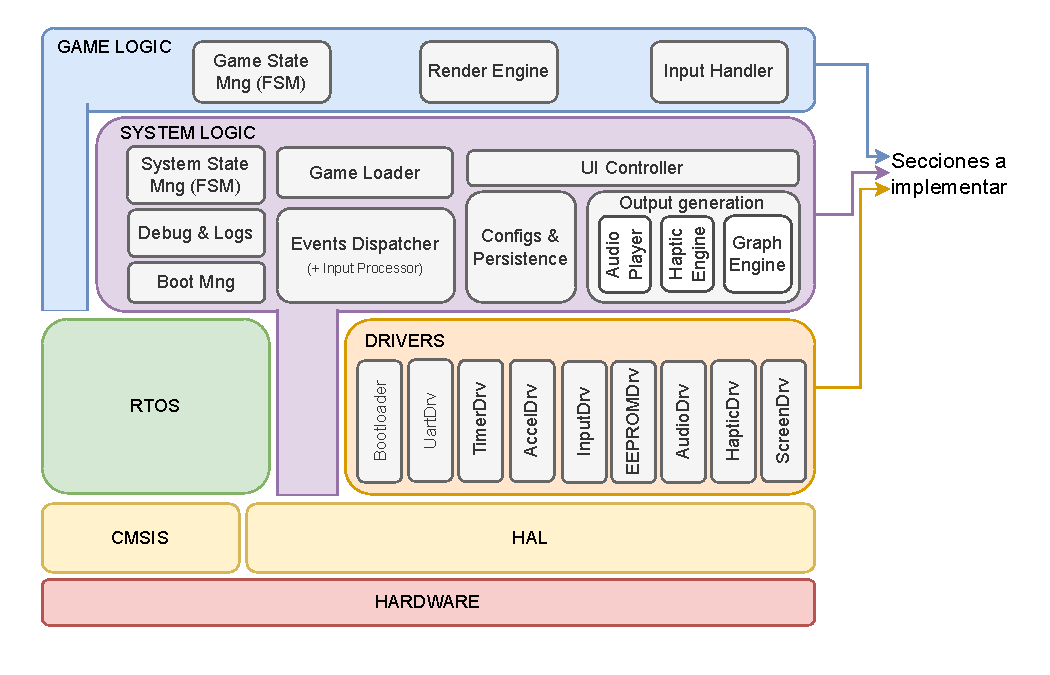
\includegraphics[width=.85\textwidth]{../Figuras/SW_layers.pdf}
\caption{Diagrama de capas del sistema.}
\label{fig:diagCapas}
\end{figure}

\subsubsection{Capa de abstracción de hardware (HAL)}
\begin{enumerate}
    \item Este patrón se utiliza cuando se desea abstraer el manejo del hardware de las funcionalidades propias de la aplicación.
    \item Se utilizará la capa de abstracción HAL provista por STM, además de incorporar una capa de drivers que la utilizará directamente para lograr una abstracción mayor hacia las capas de aplicación.
\end{enumerate}

\subsubsection{Observar y reaccionar}

\begin{figure}[htb]
\centering 
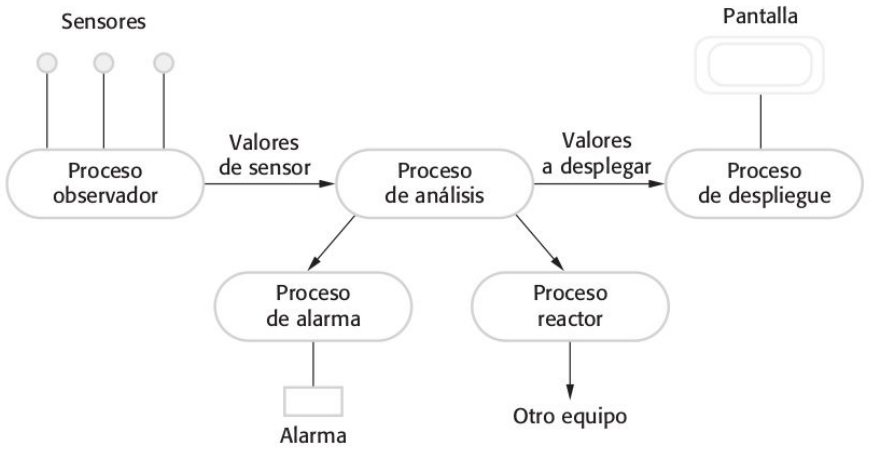
\includegraphics[width=.75\textwidth]{../Figuras/observarYreaccionar.png}
\caption{Patrón observar y reaccionar. Imagen del apunte de la materia Ingeniería de Software.}
\label{fig:obReaSYS}
\end{figure}

\begin{enumerate}
    \item Este patrón se utiliza cuando un conjunto de sensores se monitorean y despliegan una respuesta de manera rutinaria. 
    \item Este patrón describe el comportamiento del sistema en términos de procesos observadores de entradas, procesos de despliegue de salidas y un proceso central de análisis de la información y reacción apropiada. 
    \item Se aplicará este patrón de arquitectura en ambas capas de aplicación:
    \begin{enumerate}
    \item Para la capa de lógica del sistema, el proceso observador será el componente \textit{Event Dispatcher}, los procesos centrales serán \textit{System State Manager} y \textit{UI Controller}, mientras que los procesos de despliegue serán: \textit{Audio Player}, \textit{Haptic Engine} y \textit{Graph Engine}
    \item Para la capa de lógica del juego, el proceso observador será el \textit{Input Handler}, el proceso central será el \textit{Game State Manager} y el proceso de despliegue será el \textit{Render Engine}.
    \end{enumerate}
\end{enumerate}


\begin{figure}[htb]
\centering 
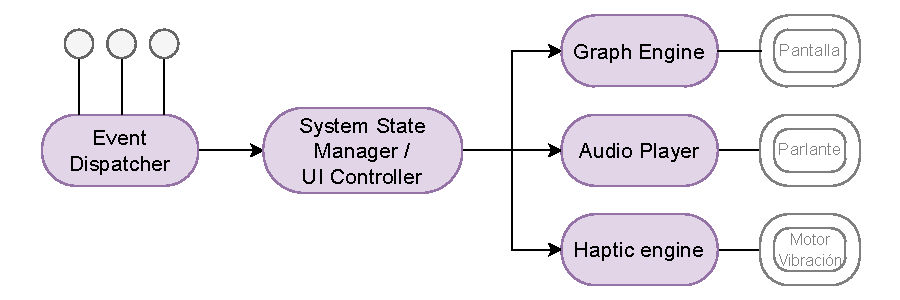
\includegraphics[width=.75\textwidth]{../Figuras/obsReac_sys.pdf}
\caption{Observar y reaccionar: patrón aplicado a la capa del sistema.}
\label{fig:obReaSYS}
\end{figure}

\begin{figure}[htb]
\centering 
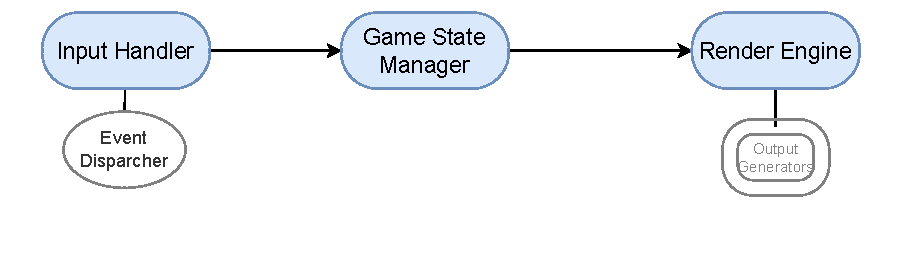
\includegraphics[width=.75\textwidth]{../Figuras/obsReac_Juego.pdf}
\caption{Observar y reaccionar: patrón aplicado a la capa del juego.}
\label{fig:obReaGAME}
\end{figure}

\subsubsection{Segmentación de procesos}
\begin{enumerate}
    \item Este patrón se usa al transformarse datos de una representación a otra antes de que puedan procesarse.
    \item Es empleado para transformar y trasladar datos a lo largo de varias etapas desacopladas mediante búferes.
    \item Será implementado para la lectura de datos, el envío de datos hacia los actuadores y las comunicaciones internas entre procesos por medio de colas y un proceso ruteador de eventos \textit{Event Dispatcher}.
\end{enumerate}

\begin{figure}[hp]
\centering 
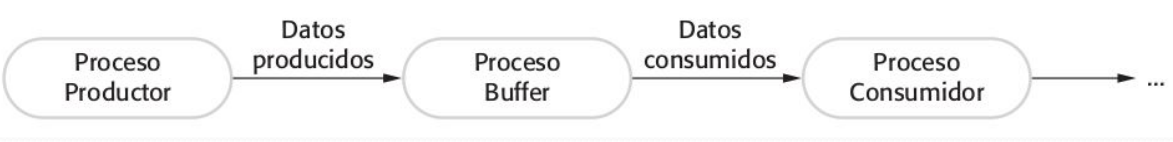
\includegraphics[width=.85\textwidth]{../Figuras/segmentacionProcesos.png}
\caption{Patrón segmentación de procesos. Imagen del apunte de la materia Ingeniería de Software.}
\label{fig:segProces}
\end{figure}

\subsection{Componentes}

%%%%%%%%%%%%%%%%%%%%%%%%%%%%%%%%%%%%%%%%%%%%%%%%%%%%%%%%%%%%
% DRIVERS                                      %
%%%%%%%%%%%%%%%%%%%%%%%%%%%%%%%%%%%%%%%%%%%%%%%%%%%%%%%%%%%%
\subsubsection{Drivers}
\begin{enumerate}
    \item Driver de acelerómetro (\texttt{AccelDrv}): lectura de acelerómetro por I\textsuperscript{2}C.
    \item Driver de memoria (\texttt{EEPROMDrv}): lectura y escritura de memoria EEPROM por SPI.
    \item Driver de pantalla (\texttt{ScreenDrv}): driver de la pantalla, gestion de ventana y transferencias DMA-SPI de píxeles.
    \item Driver de audio (\texttt{AudioDrv}): reproduce efectos de sonido mediante modulación por ancho de pulso (PWM).
    \item Driver de vibración (\texttt{HapticDrv}): comanda patrones de vibración del controlador DRV2605L mediante I\textsuperscript{2}C.
    \item Driver de UART (\texttt{UARTDrv}): comunicación serie con DMA para depuración.
    \item Driver de entradas (\texttt{InputDrv}): lectura de botones (GPIO + EXTI) y joystick (ADC DMA continuo), aplica antirrebote y dead-zone.
    \item Driver de timers (\texttt{TimerDrv}): generación de interrupciones de tiempo.
\end{enumerate}


%%%%%%%%%%%%%%%%%%%%%%%%%%%%%%%%%%%%%%%%%%%%%%%%%%%%%%%%%%%%
% LÓGICA DEL SISTEMA                                   %
%%%%%%%%%%%%%%%%%%%%%%%%%%%%%%%%%%%%%%%%%%%%%%%%%%%%%%%%%%%%
\subsubsection{Lógica del sistema}
\begin{enumerate}
    \item Boot Manager (\texttt{BootMgr}): inicialización del RTOS, creación de tareas y colas, verificación de drivers.
    \item Cargador de recursos (\texttt{ResLoader}): carga de recursos (imágenes, sonidos) en RAM desde memoria externa.
    \item Configuración y persistencia (\texttt{ConfigPersist}): guarda y carga datos de las partidas del juego en memoria externa. Verificación de partida guardada.
    \item Despachador de eventos (\texttt{EventDispatcher}): recibe eventos de bajo nivel (inputs, ticks), los normaliza y redistribuye a colas de alto nivel. Recibe y redistribuye eventos y mensajes entre componentes. 
    \item Manejador de la interfaz de usuario (\texttt{UIController}): gestión de la interfaz de usuario del sistema en los estados no interactivos del juego (menús, splash, opciones de pausa). Funciones principales:
    \begin{itemize}
      \item Construcción de las pantallas de interfaz (Splash, Menú principal, Menú de pausa).
      \item Gestión del foco y navegación de menús.
      \item Interpretación de eventos de entrada normalizados y publicación de eventos de transición de estado.
      \item Coordinación con servicios de generación de salidas para brindar retroalimentación visual, sonora y háptica.
      \item Coordinación con \texttt{ConfigPersist} para comprobar si hay partidas guardadas válidas.
      \item Acceso a recursos gráficos (iconos, textos, imágenes) mediante el \texttt{ResLoader}.
    \end{itemize}
    \item Motor gráfico (\texttt{GraphEngine}): renderizado gráfico, gestión de buffers de pantalla.
    \item Reproductor de audio (\texttt{AudioPlayer}): reproducción de efectos de sonido.
    \item Motor de retroalimentación táctil (\texttt{HapticEngine}): gestión de la activación de patrones de vibración.
    \item System State Manager (\texttt{SysMng}): implementación de máquina de estados principal del sistema, gestión de transiciones entre distintos modos de operación (\texttt{SYS\_SPLASH, SYS\_MAIN\_MENU, SYS\_IN\_GAME, SYS\_PAUSED}).
    \item Debug \& Logs (\texttt{LogSink}): gestión de comunicaciones por UART y trazas de depuración.
\end{enumerate}


%%%%%%%%%%%%%%%%%%%%%%%%%%%%%%%%%%%%%%%%%%%%%%%%%%%%%%%%%%%%
% LÓGICA DEL JUEGO                                     %
%%%%%%%%%%%%%%%%%%%%%%%%%%%%%%%%%%%%%%%%%%%%%%%%%%%%%%%%%%%%
\subsubsection{Lógica del juego}
\begin{enumerate}
    \item Game State Manager (\texttt{GameMng}): control del ciclo principal del juego, construcción del modelo gráfico del juego a partir del estado del gameplay. Manejo de los estados internos del juego (\texttt{GME\_RUNNING, GME\_FROZEN, GME\_STOPPED}).
    \item Motor de renderizado (\texttt{RenderEngine}): generación del contenido visual del juego para cada cuadro, coordinación con servicios de generación de salidas para brindar retroalimentación visual, sonora y háptica. Opera únicamente durante \texttt{GME\_RUNNING}.
    \item Gestión de entradas (\texttt{InputHandler}): traducción de los eventos normalizados de entradas del \texttt{EventDispatcher} a acciones de gameplay. Opera únicamente durante \texttt{GME\_RUNNING}.
\end{enumerate}


\subsection{Interfaces}

\subsubsection{Interfaces externas}
\begin{enumerate}
    \item \texttt{InputDrv}: botones (GPIO + EXTI) y joystick (ADC + DMA).
    \item \texttt{AccelDrv}: acelerómetro MPU-6500 I²C (400 kHz)
    \item \texttt{EEPROMDrv}: EEPROM 25LC256 SPI (10 MHz).
    \item \texttt{ScreenDrv}: ST7735 TFT, 128x160 px. SPI + DMA (48 MHz).
    \item \texttt{AudioDrv}: LM386 + audio mono 1 W (PWM / GPIO).
    \item \texttt{HapticDrv}: controlador háptico DRV2605L I²C (400 kHz).
    \item \texttt{UARTDrv}: UART + DMA (115200bps 8N1).
\end{enumerate}

\subsubsection{Interfaces internas}
\begin{enumerate}
%%%%%%%%%%%%%%%%%%%%%%%%%%%%%%%%%%%%%%%%%%%%%%%%%%%%%%%%%%%%
% DRIVERS                                      %
%%%%%%%%%%%%%%%%%%%%%%%%%%%%%%%%%%%%%%%%%%%%%%%%%%%%%%%%%%%%
  \item \texttt{InputDrv}
    \begin{enumerate}
      \item Entradas: no requiere.
      \item Salidas: datos crudos (\texttt{BTN\_X\_PRESS, \{JY\_X, JY\_Y\}}).
    \end{enumerate}
  \item \texttt{AccelDrv}
    \begin{enumerate}
      \item Entradas: no requiere.
      \item Salidas: datos crudos (\texttt{\{ACC\_X, ACC\_Y\}}).
    \end{enumerate}
  \item \texttt{EEPROMDrv}
    \begin{enumerate}
      \item Escritura:
      \begin{enumerate}
        \item Entradas: data serializada, dirección de guardado.
        \item Salidas: guardado exitoso/fallido (bool o enum).
      \end{enumerate}
      \item Lectura:
      \begin{enumerate}
        \item Entradas: dirección de lectura.
        \item Salidas: data serializada.
      \end{enumerate}
    \end{enumerate}
  \item \texttt{ScreenDrv}
    \begin{enumerate}
      \item Entradas: paquete de dibujo con bitmap RGB565 y region de pantalla a escribir (struct: \texttt{drawPacket\{x1,x2,y1,y2,bitmap\}}).
      \item Salidas: escritura de datos finalizada correctamente/fallida (bool o enum).
    \end{enumerate}
  \item \texttt{AudioDrv}
    \begin{enumerate}
      \item Entradas: frecuencia fija o muestras PCM, duración (struct: \texttt{\{*pcm, durtionMs\}}).
      \item Salidas: envío de datos finalizado correctamente/fallido (bool o enum).
    \end{enumerate}
  \item \texttt{HapticDrv}
    \begin{enumerate}
      \item Entradas: id del patrón de vibración a reproducir.
      \item Salidas: envío de datos finalizado correctamente/fallido (bool o enum).
    \end{enumerate}
  \item \texttt{UARTDrv}
    \begin{enumerate}
      \item Envío:
      \begin{enumerate}
        \item Entradas: buffer de datos a enviar.
        \item Salidas: envío de datos finalizado correctamente/fallido (bool o enum).
      \end{enumerate}
      \item Recepción:
      \begin{enumerate}
        \item Entradas: buffer de recepción de datos.
        \item Salidas: recepción de datos finalizado correctamente/fallido (bool o enum).
      \end{enumerate}
    \end{enumerate}
%%%%%%%%%%%%%%%%%%%%%%%%%%%%%%%%%%%%%%%%%%%%%%%%%%%%%%%%%%%%
% LÓGICA DEL SISTEMA                                   %
%%%%%%%%%%%%%%%%%%%%%%%%%%%%%%%%%%%%%%%%%%%%%%%%%%%%%%%%%%%%
  \item \texttt{BootMng}
    \begin{enumerate}
      \item Entradas: status de drivers inicializados (bool o enum).
      \item Salidas: señal de inicialización completa (\texttt{SYS\_READY}).
    \end{enumerate}
  \item \texttt{ResLoader}
    \begin{enumerate}
      \item Entradas: id del asset a cargar (unsigned int).
      \item Salidas: asset serializado, señal de asset disponible (\texttt{RES\_READY}).
    \end{enumerate}
  \item \texttt{ConfigPersist}
    \begin{enumerate}
      \item Existencia de partida guardada:
      \begin{enumerate}
        \item Entradas: no requiere.
        \item Salidas: partida encontrada/no encontrada (bool o enum).
      \end{enumerate}
      \item Guardar partida:
      \begin{enumerate}
        \item Entradas: partida serializada.
        \item Salidas: guardado de datos finalizado correctamente/fallido (bool o enum).
      \end{enumerate}
      \item Cargar partida:
      \begin{enumerate}
        \item Entradas: no requiere.
        \item Salidas: partida cargada/fallo en carga (bool o enum).
      \end{enumerate}
    \end{enumerate}
  \item \texttt{EventDispatcher}
    \begin{enumerate}
      \item Procesamiento de entradas:
      \begin{enumerate}
        \item Entradas: datos crudos de entradas (enum, struct: \texttt{BTN\_X\_PRESS, \{JY\_X, JY\_Y\}, \{ACC\_X, ACC\_Y\}}).
        \item Salidas: eventos normalizados de entradas (enum, struct: \texttt{BTN\_START, KEY\_UP, TILT\_RIGHT, JYcoords\{\}}).
      \end{enumerate}
      \item Despachador de eventos:
      \begin{enumerate}
        \item Entradas: eventos varios (enum, struct).
        \item Salidas: eventos reenviados (enum, struct).
      \end{enumerate}
      \item Activar/desactivar trazas de depuración:
      \begin{enumerate}
        \item Entradas: señal de traza activada/desactivada (bool o enum).
        \item Salidas: no emite.
      \end{enumerate}
    \end{enumerate}
  \item \texttt{UIController}
    \begin{enumerate}
      \item Entradas: eventos varios (enum, struct).
      \item Salidas: 
      \begin{itemize}
        \item eventos de transición de estado del sistema y del juego (enum).
        \item datos para reproducción de audio (struct: \texttt{\{id, duration\}}).
        \item datos para generación de vibración (enum: \texttt{SEND\_PATTERN\_1, SEND\_PATTERN\_2}).
        % \item modelo de juego para motor gráfico (struct: \texttt{gameModel\{\}}).
        \item lista de objetos gráficos (struct: \texttt{drawList\{\}}).
      \end{itemize}
    \end{enumerate}
  \item \texttt{GraphEngine}
    \begin{enumerate}
        \item Entradas: lista de objetos gráficos (struct: \texttt{drawList\{\}}).
        \item Salidas: 
        \begin{itemize}
          \item listas de dibujo para el driver de pantalla (struct: \texttt{drawPacket\{x1,x2,y1,y2,bitmap\}}).
          \item envío de datos finalizado correctamente/fallido (bool o enum).
        \end{itemize}
    \end{enumerate}
  \item \texttt{AudioPlayer}
    \begin{enumerate}
      \item Entradas: datos de audio (struct: \texttt{audioCue\{id, duration\}}).
      \item Salidas: 
      \begin{itemize}
        \item audio para el driver (struct: \texttt{\{*pcm, durtionMs\}}).
        \item envío de datos finalizado correctamente/fallido (bool o enum).
      \end{itemize}
      envío de datos finalizado correctamente/fallido (bool o enum).
    \end{enumerate}
  \item \texttt{HapticEngine}
    \begin{enumerate}
      \item Entradas: datos de vibración (enum: \texttt{hapticCue: SEND\_PATTERN\_1, SEND\_PATTERN\_2}).
      \item Salidas: 
      \begin{itemize}
        \item id del patrón de vibración a reproducir por el driver de vibración.
        \item envío de datos finalizado correctamente/fallido (bool o enum).
      \end{itemize}
    \end{enumerate}
  \item \texttt{SysMng}
    \begin{enumerate}
      \item Entradas: eventos de transición de estado del sistema (enum).
      \item Salidas: 
      \begin{itemize}
        \item eventos de transición del juego (enum).
        \item señales de cambio de estado confirmado para renderizado de menús (struct).
      \end{itemize}
    \end{enumerate}
  \item \texttt{LogSink}
    \begin{enumerate}
      \item Recepción de comandos:
      \begin{enumerate}
        \item Entradas: comando recibido por UART.
        \item Salidas: señal de traza activada/desactivada (bool o enum).
      \end{enumerate}
      \item Reenvío de logs de depuración:
      \begin{enumerate}
        \item Entradas: eventos del \texttt{EventDispatcher}.
        \item Salidas: eventos en buffer de datos a enviar por UART.
      \end{enumerate}
    \end{enumerate}
%%%%%%%%%%%%%%%%%%%%%%%%%%%%%%%%%%%%%%%%%%%%%%%%%%%%%%%%%%%%
% LÓGICA DEL JUEGO                                     %
%%%%%%%%%%%%%%%%%%%%%%%%%%%%%%%%%%%%%%%%%%%%%%%%%%%%%%%%%%%%
  \item \texttt{InputHandler}
    \begin{enumerate}
      \item Entradas: eventos normalizados de entradas (enum, struct).
      \item Salidas: 
      \begin{itemize}
        \item acciones de gameplay (enum).
        \item señal de detección de pausa de juego.
      \end{itemize}
    \end{enumerate}
  \item \texttt{RenderEngine}
    \begin{enumerate}
      \item Entradas: 
      \begin{itemize}
        \item modelo gráfico de juego (struct: \texttt{gameModel\{\}}).
        \item lista de hechos relevantes del juego (array: \texttt{gameSignal[]}).
      \end{itemize}
      \item Salidas: 
      \begin{itemize}
        \item datos para reproducción de audio (struct: \texttt{audioCue\{audio\_id, duration\}}).
        \item datos para generación de vibración (enum: \texttt{hapticCue: SEND\_PATTERN\_1, SEND\_PATTERN\_2}).
        \item lista de objetos gráficos para el motor de gráficos (struct: \texttt{drawList\{\}}).
      \end{itemize}
    \end{enumerate}
  \item \texttt{GameMng}
    \begin{enumerate}
      \item Actualización del estado del juego:
      \begin{enumerate}
        \item Entradas: eventos de transición del estado del juego (enum).
        \item Salidas: no requiere.
      \end{enumerate}
      \item Procesamiento de acciones:
      \begin{enumerate}
        \item Entradas: acciones de gameplay (enum).
        \item Salidas:
        \begin{itemize}
          \item lista de hechos relevantes del juego (array: \texttt{gameSignal[]}).
          \item modelo gráfico de juego (struct: \texttt{gameModel\{\}}).
        \end{itemize}
      \end{enumerate}
    \end{enumerate}
  \end{enumerate}

\begin{sidewaysfigure}[hp]
  \centering
  % Como la página está girada 90°, es mejor usar \textheight
  % para que llene lo máximo posible.
  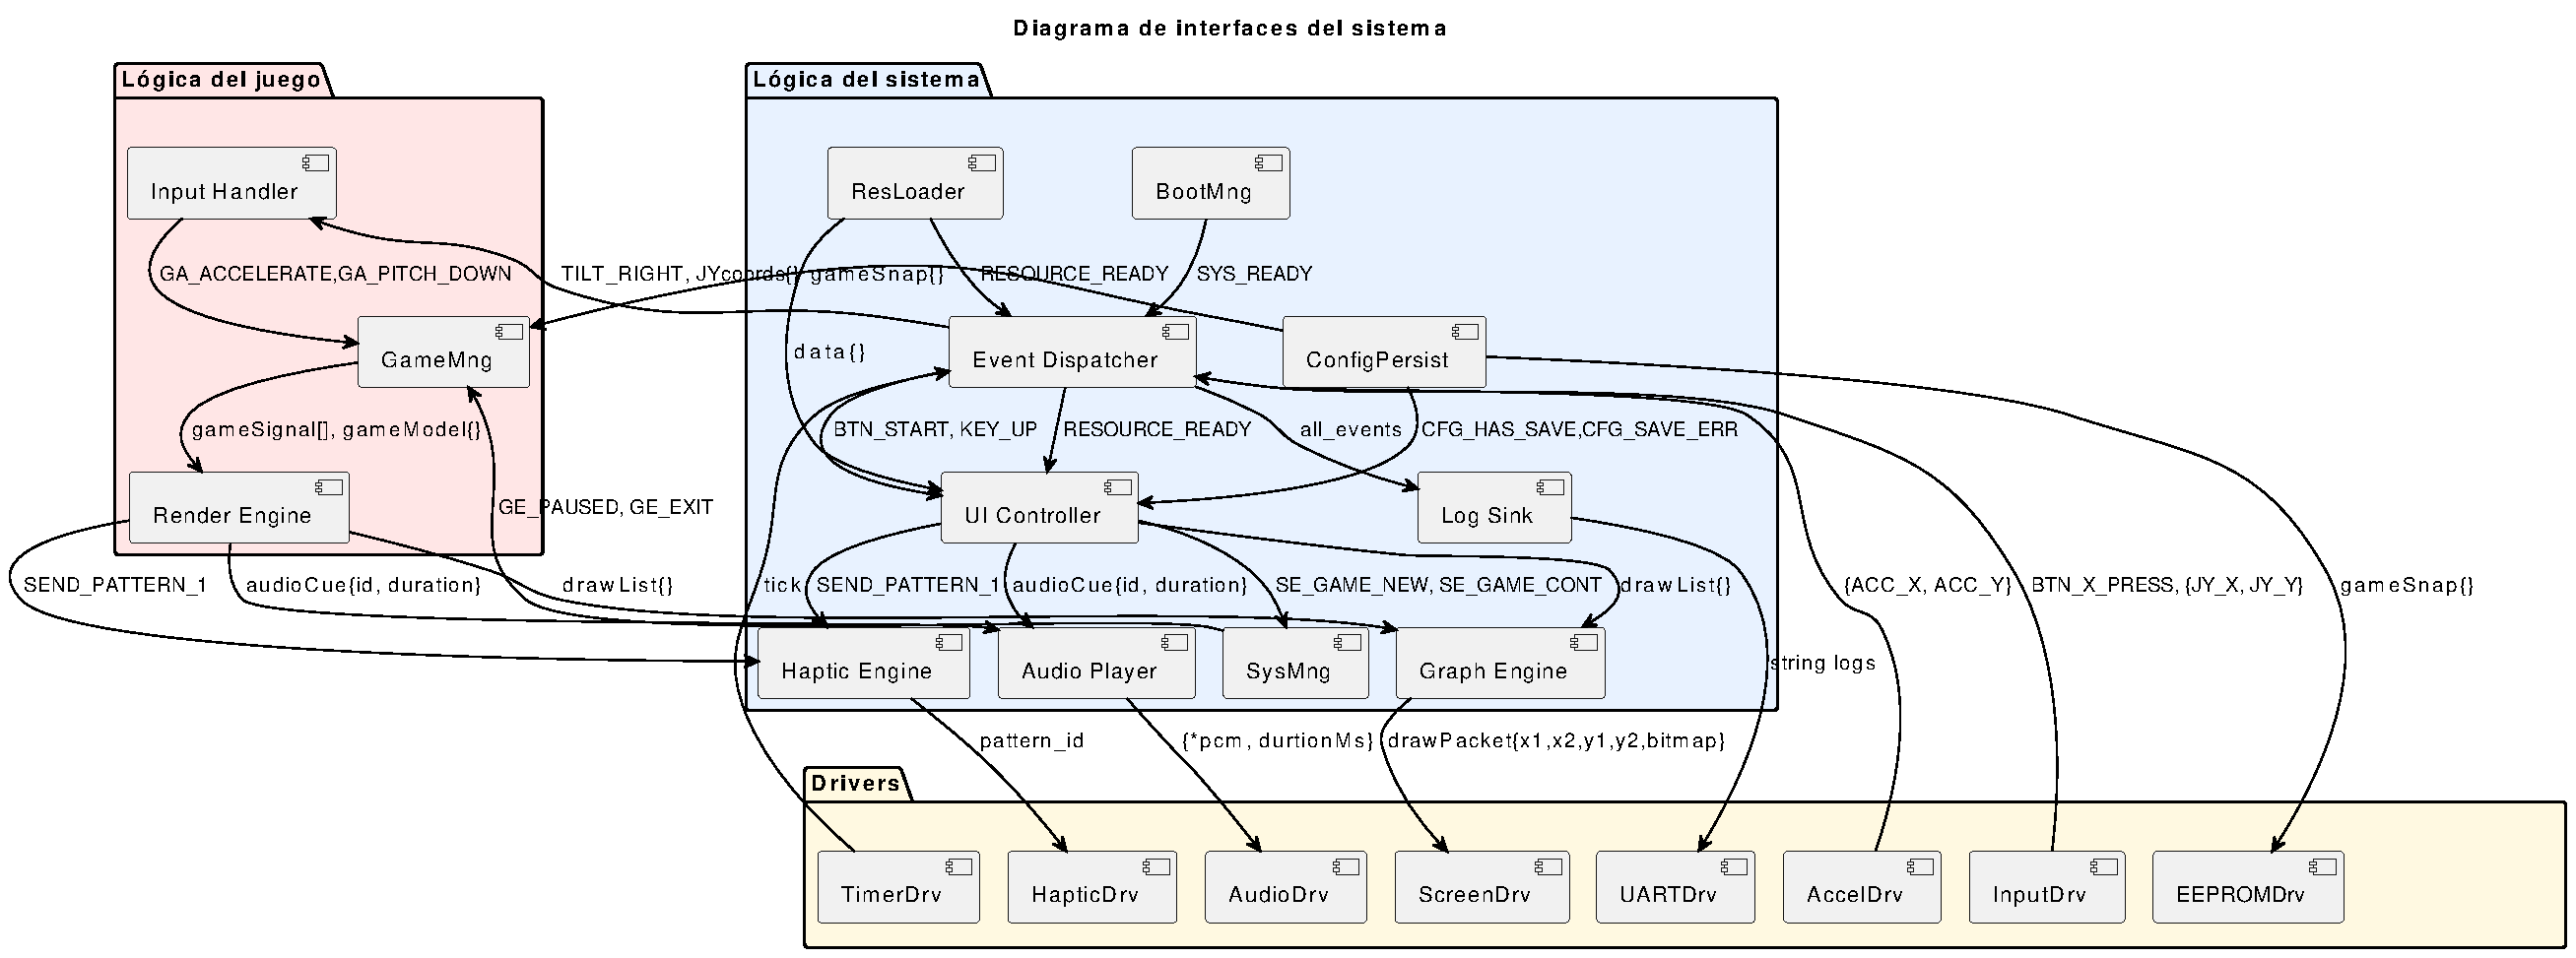
\includegraphics[width=.95\textheight]{../Figuras/diagrama_interfaces.pdf}
  % \caption{Diagrama de interfaces del sistema.}
  \label{fig:diagInterfaz}
\end{sidewaysfigure}

% \begin{figure}[htb]
% \centering 
%   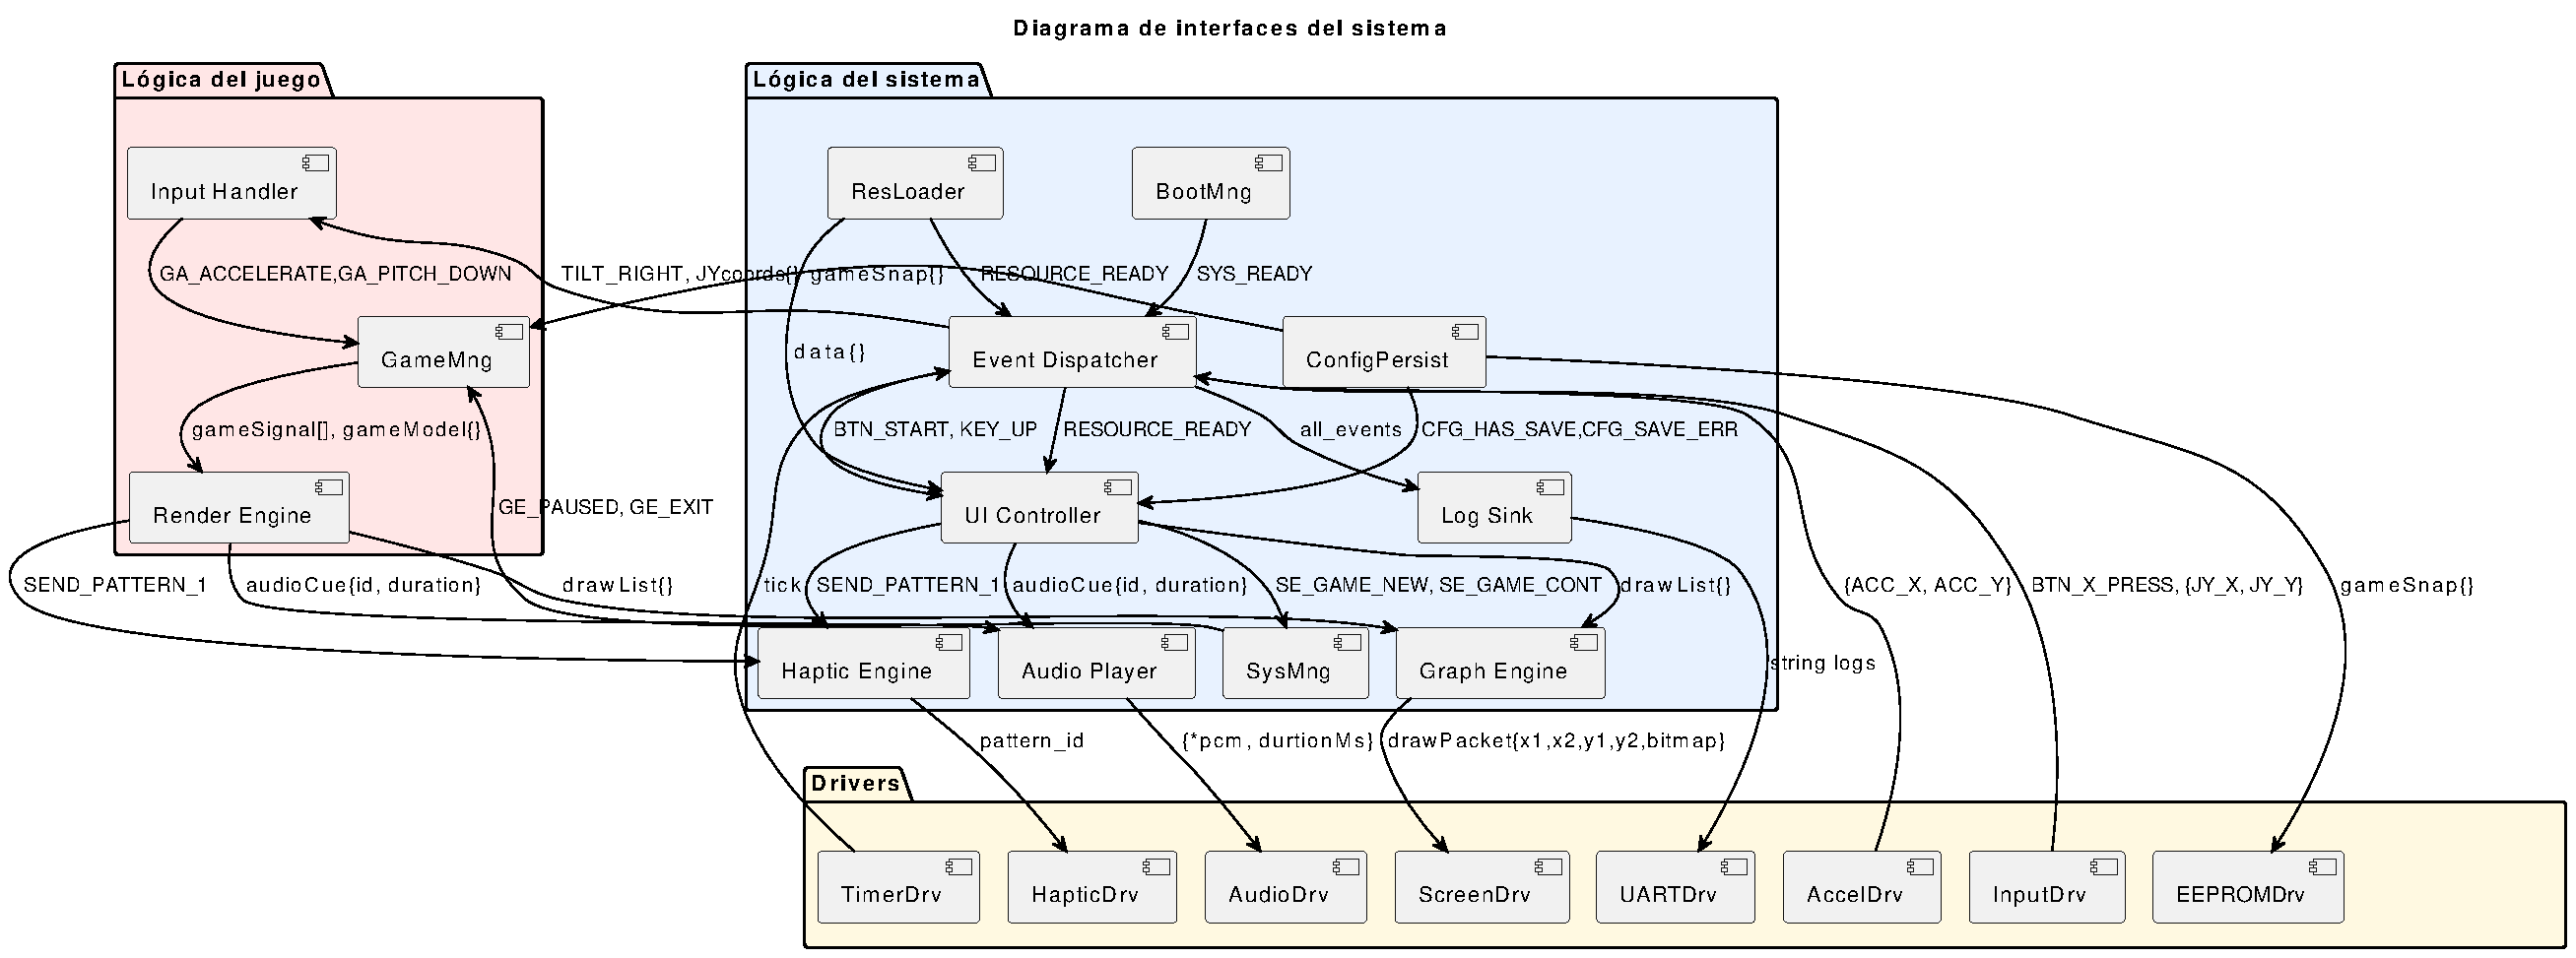
\includegraphics[width=.95\textwidth]{../Figuras/diagrama_interfaces.pdf}
%   % \caption{Diagrama de interfaces del sistema.}
%   \label{fig:diagInterfaz}
% \end{figure}


% @startuml
% !pragma layout smetana
% '!pragma layout
% top to bottom direction

% skinparam rectangle {
%   BackgroundColor #FDF6E3
%   BorderColor Black
% }
% 'skinparam linetype ortho
% skinparam arrow {
%   Color Black
%   Thickness 1
% }

% skinparam component<<anchor>> {
%   BackgroundColor transparent
%   BorderColor     transparent
%   FontColor       transparent
% }

% title Diagrama de interfaces del sistema


% package "Lógica del juego" #FFE6E6 {
%   [Input Handler]
%   [GameMng]
%   [Render Engine]
%   component LGanchor <<anchor>> 
% }


% package "Lógica del sistema" #E8F2FF {
%   [Event Dispatcher]
%   [UI Controller]
%   [SysMng]
%   [Graph Engine]
%   [Audio Player]
%   [Haptic Engine]
%   [ResLoader]
%   [ConfigPersist]
%   [Log Sink]
%   [BootMng]
%   component SYSanchor <<anchor>>
% }
% LGanchor -[hidden]-> SYSanchor

% package "Drivers" #FFF9E1 {
%   [InputDrv]
%   [AccelDrv]
%   [EEPROMDrv]
%   [ScreenDrv]
%   [AudioDrv]
%   [HapticDrv]
%   [UARTDrv]
%   [TimerDrv]
%   component DRVanchor <<anchor>>
% }

% SYSanchor -[hidden]-> DRVanchor
% 'LGanchor -[hidden]-> DRVanchor

% InputDrv -up-> [Event Dispatcher] : BTN_X_PRESS, {JY_X, JY_Y}
% AccelDrv -up-> [Event Dispatcher] : {ACC_X, ACC_Y}

% ConfigPersist --> EEPROMDrv : gameSnap{}
% [Graph Engine] --> ScreenDrv : drawPacket{x1,x2,y1,y2,bitmap}
% [Audio Player] --> AudioDrv : {*pcm, durtionMs}
% [Haptic Engine] --> HapticDrv: pattern_id
% BootMng --> [Event Dispatcher]: SYS_READY
% [TimerDrv]-up-> [Event Dispatcher]: tick
% [Event Dispatcher] --> [UI Controller] : BTN_START, KEY_UP
% [Event Dispatcher] --> [Input Handler] : TILT_RIGHT, JYcoords{}

% [Event Dispatcher] --> [Log Sink]: all_events

% [ResLoader] --> [UI Controller] : data{}
% [ResLoader] --> [Event Dispatcher]: RESOURCE_READY
% [Event Dispatcher] --> [UI Controller]: RESOURCE_READY

% [ConfigPersist] --> [GameMng] : gameSnap{}
% [ConfigPersist] --> [UI Controller] : CFG_HAS_SAVE,CFG_SAVE_ERR

% [UI Controller] --> [SysMng] : SE_GAME_NEW, SE_GAME_CONT
% [UI Controller] --> [Audio Player]: audioCue{id, duration}
% [UI Controller] --> [Haptic Engine]: SEND_PATTERN_1
% [UI Controller] --> [Graph Engine] : drawList{}
% [SysMng] --> [GameMng]: GE_PAUSED, GE_EXIT

% [Input Handler] --> [GameMng] : GA_ACCELERATE,GA_PITCH_DOWN

% [GameMng] --> [Render Engine] : gameSignal[], gameModel{}
% [Render Engine] --> [Graph Engine] : drawList{}

% [Render Engine] --> [Audio Player]: audioCue{id, duration}
% [Render Engine] --> [Haptic Engine]: SEND_PATTERN_1

% [Log Sink] --> UARTDrv : string logs
% @enduml


% ============================================================
% \appendix
% \section{Glosario de interfaces}
% \begin{description}[leftmargin=1cm,labelindent=0.5cm]
%   \item[\textbf{event\_t}] estructura de 8 bytes: \verb|uint8_t type; uint8_t arg0; uint16_t arg1; uint32_t ts;|
%   \item[\textbf{sprite\_t}] índice de textura, x, y, flags (4 bytes).
% \end{description}

\end{document}
